\chapter{First Use}
\label{chap:firstuse}
 
\section{Installing the Toolbox}
\label{sec:installation}

Once the toolbox has been download and extracted, it can be installed by running the file ``\textit{install.m}'' in the root folder. This adds all the toolbox folders to the search path of Matlab. Additionally, the installation script checks for the presence of any required external library. Currently, $3$ libraries are needed by the toolbox: LibSVM\footnote{\url{http://www.csie.ntu.edu.tw/~cjlin/libsvm/}}, the DeepLearn Toolbox\footnote{\url{https://github.com/rasmusbergpalm/DeepLearnToolbox}}, and the Kernel Methods Toolbox\footnote{\url{http://sourceforge.net/projects/kmbox/}}. None of them is essential, but some specific algorithms depend on them. If a library is not found, the installation script asks for the permission of downloading it and storing it in the ``lib'' folder:

\begin{console}
Checking for presence of Deep Learn Toolbox...
Deep Learn Toolbox not found. Do you want to install it? (Y/N) 
\end{console}

\noindent If the user denies the permission, the installation process continues, but the functionalities depending on the external library cannot be used. In this example, if the user denies the permission to install the DeepLearn Toolbox, a warning message will tell us that the \textit{StackedAutoEncoder} algorithm depends on it:
 
\begin{console}
Deep Learn Toolbox not found. Do you want to install it? (Y/N) N
You will not be able to use the StackedAutoEncoder algorithm
\end{console}
 
\noindent Due to the presence of a large set of folders, the search path is not saved by default. Hence, the installation script must be run every time Matlab is restarted. Alternatively, it is possible to save the path after the installation by running the built-in ``\textit{savepath}'' command. 

\section{Folder Structure}
\label{sec:folders}

Before continuing, let us look briefly at the folder structure of \toolboxname after the installation process. In Fig. \ref{fig:folders} we show a unix-like representation of the directories, together with a brief comment on their contents.

\begin{figure}[h]
\dirtree{%
.1 /.
.2 configs\DTcomment{Configuration files}. 
.2 core. 
.3 classes\DTcomment{Core classes of the toolbox}. 
.3 functions\DTcomment{Core functions of the toolbox}. 
.2 datasets\DTcomment{Available datasets}. 
.3 R. 
.3 BC. 
.3 (others). 
.2 functionalities\DTcomment{User-defined algorithms, etc.}. 
.3 algorithms. 
.3 performance. 
.3 preprocessors. 
.3 wrappers. 
.2 help\DTcomment{Help scripts for HTML reports}. 
.2 lib\DTcomment{External libraries}.
.2 manual\DTcomment{This manual folder}. 
.2 results\DTcomment{Saved results}. 
.2 scripts\DTcomment{Output scripts}. 
.2 tests\DTcomment{Testing suite}. 
.2 tmp\DTcomment{Temporary folder}. 
}
\label{fig:folders}
\caption{Folder Structure of the Toolbox}
\end{figure} 

\noindent Most of the directories contents are self-explanatory and will be explored in depth in the rest of this manual, but some general comments are in order. First, datasets are partitioned into multiple subfolders, corresponding to the internal concept of ``\textit{task}'', introduced in Section \ref{sec:understandingtasks}. All the user-defined functionalities, which can be roughly subdivided into $4$ families (learning algorithms, performance measures, preprocessors and wrappers) are stored in the corresponding subfolder of ``\textit{functionalities}''. Note that the toolbox already comes with several ready-to-use implementations and datasets. To get a general overview at the currently available functionalities and datasets, help scripts in the \textit{help} folder can be used to generate HTML reports. Internally, this is done using the Matlab Report Generator\footnote{\url{http://www.mathworks.it/products/ML_reportgenerator/}}. Output scripts are used for showing additional information after the simulation, and are introduced in Section \ref{sec:outputscripts}. The temporary folder is emptied at the end of every simulation, and whenever Matlab is closed. Finally, the toolbox is supplemented by a suite of unitary tests for checking the correctness of the code. This suite should be run every time a change is made to the code of the toolbox.

\section{General Workflow}

\begin{figure}
\centering
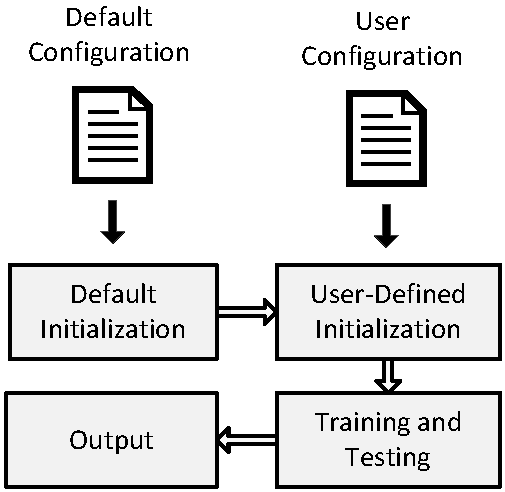
\includegraphics[scale=0.6]{./images/Workflow}
\caption{High-level Schema of the Execution of the Toolbox}
\label{fig:workflow}
\end{figure}

The general workflow of the toolbox is depicted in Fig. \ref{fig:workflow}. The simulation starts by loading a default configuration, saved in ``\textit{configs/default\_config.m}''. Then, the user-defined configuration is loaded, corresponding to the file ``\textit{config.m}'' in the root folder of the toolbox. In this file, the user can specify what algorithms must be tested, and on which datasets. Additionally, it is possible to override some general behavior of the toolbox, and to enable some advanced features, such as parallelization of the experiments.

According to these requirements, the toolbox trains and tests a set of models on the requested data, and at the end shows on the console the average training times and testing accuracies. To understand briefly the training phase, consider the simplest case of a single algorithm, tested on a single dataset, using a random partition of the data. The worflow of execution is detailed in Fig. \ref{fig:trainingphase}. The dataset is loaded from memory and preprocessed using a set of methods specified in the configuration file. Then, the preprocessed dataset is subdivided into a training set and a testing set. The training set is then passed in input to a learning algorithm, to build a suitable model. The learning algorithm can be encapsulated into one (or more) wrappers, allowing for the possibility of fine-tuning its parameters, choosing the right subset of input features, and many additional functionalities. Finally, the testing set is passed as input to the model, which provides a set of predicted outputs. This outputs are compared with the expected ones using a given measure of accuracy, that determines the final testing error of the algorithm. All the blocks of Fig. \ref{fig:trainingphase} are fully configurable and extensible.

\begin{figure}
\centering
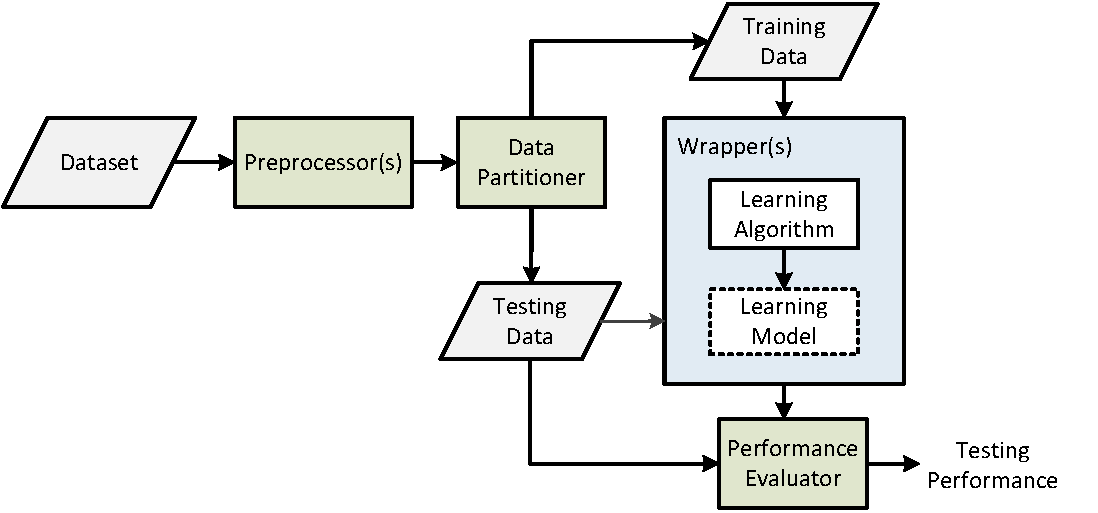
\includegraphics[scale=0.75]{./images/Disegno3}
\caption{Schematic Depiction of the Training Phase}
\label{fig:trainingphase}
\end{figure}

In the more general case, the data can be split according to a $k$-fold cross validation, hence the training/testing process is repeated $k$ times and results are averaged. This can be repeated for multiple algorithms and datasets, although the preprocessing step and the partitioning steps are common to all the algorithms so as to ensure a fair comparison. Additionally, the overall process can be repeated multiple times (\textit{runs}).

\section{Running the First Test}
\label{sec:runningfirsttest}
To help familiarizing with the software, the configuration file already contains the instructions to run a very simple experiment. 
Although its syntax is explored in detail in the following chapter, for the sake of this demo it is enough to understand that this example requires the test of two different learning algorithms:

\begin{lstlisting}
add_algorithm('B', 'Baseline', @Baseline);
add_algorithm('ELM', 'Extreme Learning Machine', @ExtremeLearningMachine);
\end{lstlisting}

\noindent The ``baseline'' algorithm is a dummy learning algorithm who, in this case, always outputs the mean value of its training set. The second algorithm is a more sophisticated Extreme Learning Machine trained using an $L2$-regularized ridge regression \cite{Huang2012}. The test is executed on a single dataset taken from the UCI repository\footnote{\url{http://archive.ics.uci.edu/ml/}}:

\newpage

\begin{lstlisting}[language=matlab]
add_dataset('G', 'Glass', 'uci_glass');
\end{lstlisting}

\noindent In this case, we have no wrappers and no preprocessors. The simulation is started by executing the ``\textit{run\_simulation.m}'' script in the root folder. The result of the simulation is then printed on the console. Below we provide a small description of each phase.

\subsection{Initialization Phase}

In the initialization phase, the configuration file is read and all the data structures are initialized:

\begin{console}
Initializing simulation...
Current seed for prng: 1340863332
End of initialization, will test 2 algorithm(s) on 1
   dataset(s) for 1 time(s)
\end{console}

\noindent Other preliminary actions are eventually run in this phase. For example, the toolbox checks the compatibility of all the algorithms with the requested datasets (see next section); it activates a pool of threads if parallelization is requested; and so on.

\subsection{Training Phase}

In the training phase, each algorithm is run on every dataset in turn. In this case, the default configuration specifies to execute a $3$-fold cross validation, and a single run:

\begin{console}
Testing Extreme Learning Machine on Glass (run 1/1)
   Fold 1... 
   Fold 2... 
   Fold 3... 
Testing Baseline on Glass (run 1/1)
   Fold 1... 
   Fold 2... 
   Fold 3... 
\end{console}

\subsection{Output Phase}
\label{sec:outputphase}

In the output phase, the results, in the form of mean and standard deviation of the errors and the training times, are printed on screen. As an example, these are typical average errors for the demo:

\begin{console}
Average error:
       Baseline  Extreme Learning Machine
Glass     1.014                    0.5375
\end{console}

Note that the actual meaning of the numbers may vary depending on the dataset. This is explained in more detail in the next section.

After this step, an optional statistical testing is executed. See Section \ref{sec:statistical_testing} for information on how to request it. Currently supported statistical tests include a Wilcoxon signed rank test \cite{dietterich1998approximate}, and a Friedman test \cite{demvsar2006statistical}. Additional output scripts can be added to the simulation for gathering information on the run. This functionality is explored in Section \ref{sec:outputscripts}.

\section{Understanding Tasks and Analyzing the Output}
\label{sec:understandingtasks}

\vspace{-2em}

\begin{center}
\begin{table}
{\centering\hfill{}
\begin{tabular}{lll}
\toprule
ID & Input & Output \\ 
\midrule
R (Regression) & \multirow{3}{*}{$\vect{X} \in \R^{N \times d}$ } & $\vect{y} \in \R^N$ \\
BC (Binary Classification) & & $\vect{y} \in \left\{-1,+1\right\}^N$\\
MC (Multiclass Classification) & & $\vect{y} \in \left\{1,\dots,M\right\}^N$\\
\bottomrule
\end{tabular}}
\hfill{}
\caption{Summary of the basic tasks defined in the toolbox}
\label{tab:basictasks}
\end{table}
\end{center}

\subsection{Basic Tasks}

To understand the results, a few more details on the structure of the toolbox is required. Speaking broadly, a dataset is composed of an $N \times d$ matrix of real values (currently, categorical variables are not supported), and a $N \times 1$ vector of targets, where $N$ is the number of examples available to the system, and $d$ is the input dimensionality. That is, each row in the input matrix is an observation, whereas each column is a feature.

A \textit{task} identifies the type of learning problem of a given dataset, which changes the type of the requested output. The following basic tasks are currently defined:

\begin{description}
\item[Regression (R)]: the output is a single real number.
\item[Binary Classification (BC)]: the output is an integer number in the set $\left\{-1,+1\right\}$.
\item[Multiclass Classification (MC)]: the output is an integer number in the set $\left\{1,\dots,M\right\}$, where $M$ is the number of classes.
\end{description} 
	
These are summarized in Table \ref{tab:basictasks}. An algorithm can be defined to work on one or more of them. For example, a particular algorithm can be defined only for classification tasks, i.e. BC and MC tasks, but not for regression tasks. If in the simulation some inconsistencies are found (i.e., an algorithm is tested on an unsupported task), they are listed in the beginning and the statistical testing is avoided. The following is an example of the corresponding warning message:

\begin{console}
The following tests are not possible:
	 KRLS on Yeast.
Statistical testing will not be executed.
\end{console}

\noindent Successively, the corresponding training phase is skipped:

\begin{console}
Testing KRLS on Yeast (run 1/1)
	Not Allowed
\end{console}

\subsection{Complex Tasks}

\vspace{-2em}

\begin{center}
\begin{table}[t]
{\centering\hfill{}
\begin{tabular}{llll}
\toprule
ID & Input & Output \\ 
\midrule
PR (Prediction) & $\vect{x} \in \R^N$ & NA \\
ML (Multilabel Classification) & $\vect{X} \in \R^{N \times d}$ & $\left\{ \vect{y}_i \right\}, \vect{y}_i = \left\{-1, +1\right\}^N$ \\
\bottomrule
\end{tabular}}
\hfill{}
\caption{Summary of the complex tasks defined in the toolbox}
\label{tab:complextasks}
\end{table}
\end{center}

Clearly, the tasks of Table \ref{tab:basictasks} do not cover all the possibilities arising in supervised learning. For this reason, the toolbox identifies a set of non-basic tasks, i.e., tasks that do not conform to the previous description. Practically, what changes is either the semantic of the problem, or the way in which the data is stored on the disk. A non-basic task is handled by previously transforming it into one or more basic tasks. Currently, two non-basic tasks are defined: 

\begin{description}
\item[Prediction (PR)]: here the input is a vector containing the ordered samples of a time-invariant time series, and the required output is a one-step ahead prediction. This is handled by transforming it into a regression problem, where the input is an embedding of the previous $r$ values of the time-series, with $r$ specified by the user. If the time series has $N$ values, $N-r$ examples are constructed.

\item[Multilabel (ML)]: this is the case where a given number $T$ of binary classification problems are defined on the same input matrix. This is handled by constructing $T$ separate binary classification tasks during the initialization phase.
\end{description}

The structure of each complex task is summarized in Table \ref{tab:complextasks}. In Table \ref{tab:correspondeces}, instead, we show how each complex task is handled by the toolbox.

\begin{center}
\begin{table}[t]
{\centering\hfill{}
\begin{tabular}{ll}
\toprule
Original Task & Transformed Tasks \\ 
\midrule
PR & A single R task.  \\
ML & Multiple BC tasks. \\
\bottomrule
\end{tabular}}
\hfill{}
\caption{Transformations between Complex Tasks and Basic Tasks}
\label{tab:correspondeces}
\end{table}
\end{center}

\subsection{Training Performance}

The measure of performance shown in the results changes depending on the task associated to each dataset. By default, the misclassification rate is shown for classification tasks, while the Normalized Root Mean-Squared error \footnote{\url{http://en.wikipedia.org/wiki/Root-mean-square_deviation}} for regression, defined as:

\begin{equation}
\text{NRMSE}(\vect{y}, \vect{d}) = \sqrt{\frac{\sum_{i=1}^N (d_i-y_i)^2}{N \hat{\sigma}_y}}
\label{eq:nrmse}
\end{equation}

\noindent where $\vect{y}$ are the expected outputs, $\vect{d}$ are the actual outputs, $N$ is the cardinality of both $\vect{y}$ and $\vect{d}$, and $ \hat{\sigma}_y$ is an empirical estimate of the variance of $\vect{y}$. The measure of error is averaged over all the folds and all the runs.

As an example, consider the sample run of Section \ref{sec:outputphase}. Since the Glass dataset is a regression task, the numbers that appear in the console are the NRMSE computed over the testing set, averaged over the different folds. The default performance measures can be changed by the user, a functionality explored in Section \ref{sec:changingperformance}. Also, new performance measures can be defined, see Section \ref{sec:implementingperformancemeasures}. 
